\subsection{Piloto AWS Industrial}
\label{subsec:aws-industrial2}

Industrial somete la arquitectura a modos de fallo que la campaña Cargo, con una sola carga, no expone. La escena modificada toma como procedencia el almacén de AWS RoboMaker, cuyo repositorio oficial se distribuye bajo licencia MIT-0 \parencite{awsRobomakerWarehouse2021}. Contiene \AwsSceneRobots{} AMR, \AwsSceneActiveLoads{} cargas activas, \AwsSceneQueuedLoads{} en cola y tráfico controlado (Figura~\ref{fig:aws-industrial2-scene}). Sensado y comunicación usan radios \AwsSceneSensingRadius{} y \AwsSceneCommunicationRadius{}~m. El acoplamiento cinemático omite agarre, fricción, tracción, \emph{wrench} y dinámica 3D.

\begin{figure}[!htbp]
  \centering
  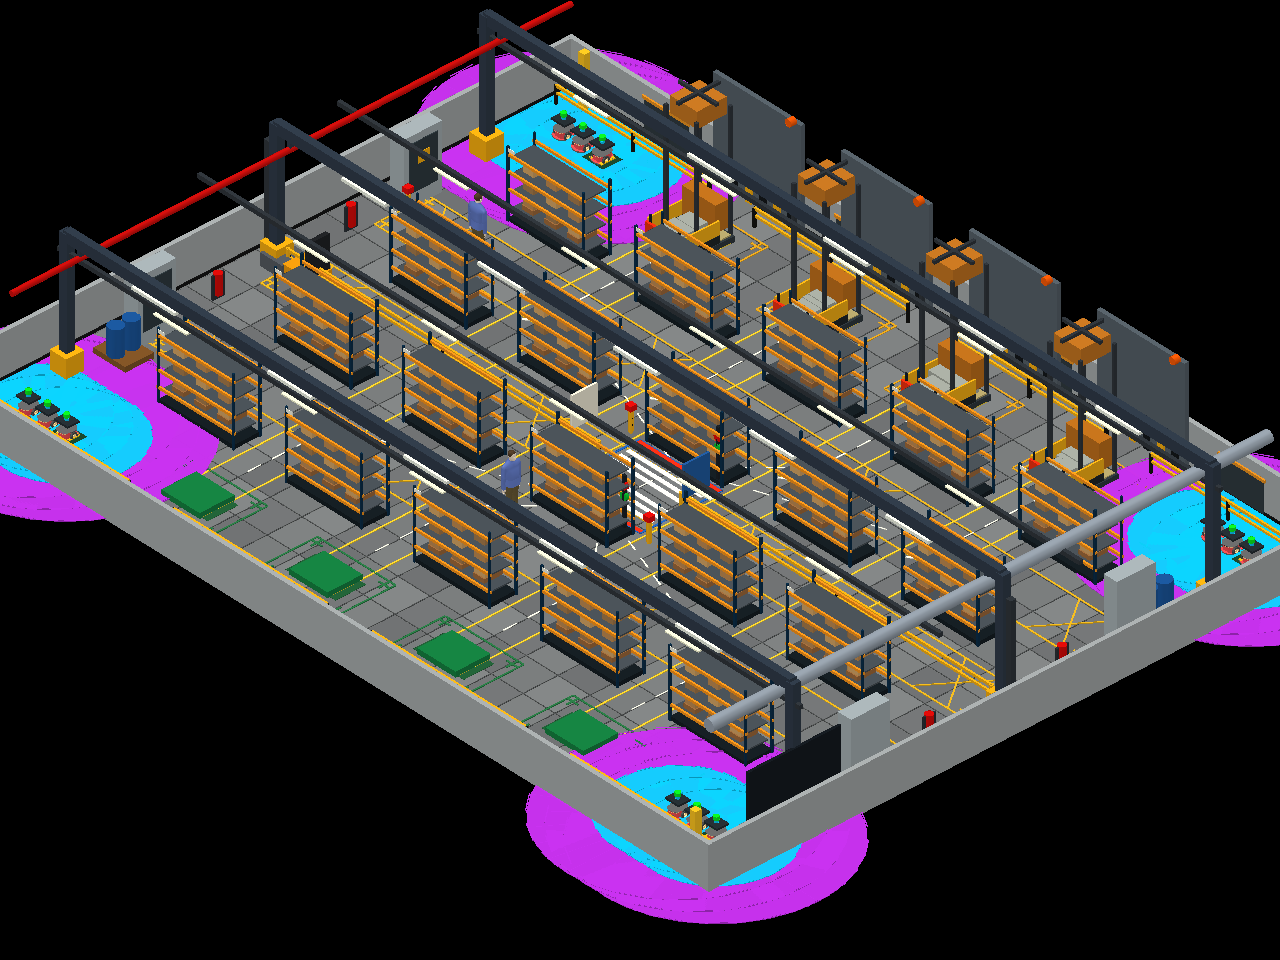
\includegraphics[width=0.50\textwidth]{../results/coppeliasim_validation/aws_industrial_adversarial_industrial2/aws_industrial_oblique_camera.png}
  \caption{Vista depurada de AWS Industrial 2 usada como piloto geométrico y cinemático. La limpieza visual no altera las huellas operacionales auditadas.}
  \label{fig:aws-industrial2-scene}
  \viusource{elaboración propia sobre la escena AWS RoboMaker Small Warehouse World, modificada para este TFM \parencite{awsRobomakerWarehouse2021}}
\end{figure}

Se cruzaron cuatro métodos, cuatro escenarios y dos semillas: \AwsPilotRuns{} ejecuciones de \AwsPilotHorizon{}~s. La referencia central usa un MILP instantáneo global sin planificación espacio--temporal. Subasta, reciprocidad y predictor son \emph{proxies} que no reproducen CBBA, ORCA o DMPC. Solo el centro abierto produjo entregas. Central MILP + preview obtuvo \AwsOpenCentralDeliveries{}, Auction + reciprocal proxy \AwsOpenAuctionDeliveries{}, Auction + predictive CBF proxy \AwsOpenPredictiveDeliveries{} y Replicator + CBF (TFM) \AwsOpenTfmDeliveries{} cargas por ejecución. Los otros tres escenarios obtuvieron cero. La referencia central optimiza la asignación de cada instantánea, pero no anticipa las reservas espacio--temporales. Su valor \AwsOpenCentralDeliveries{} documenta un bloqueo del ejecutor integrado y no un fallo del MILP de asignación.

Las 32 ejecuciones no registraron solapamientos muestreados, pero Replicator--CBF permaneció bloqueado durante una fracción \AwsTfmDeadlockMin{}--\AwsTfmDeadlockMax{} del tiempo simulado, según el clasificador operacional del piloto. La separación geométrica no implica vivacidad. Dos semillas no permiten establecer un ranking ni estimar fiabilidad industrial.
